% *********************************************************************
% © 2021-2022 Jeremy Sylvestre
%
% Permission is granted to copy, distribute and/or modify this document
% under the terms of the GNU Free Documentation License, Version 1.3 or
% any later version published by the Free Software Foundation; with no
% Invariant Sections, no Front-Cover Texts, and no Back-Cover Texts. A
% copy of the license is included in the appendix entitled “GNU Free
% Documentation License” that appears in the output document of this
% PreTeXt source code. All trademarks™ are the registered® marks of
% their respective owners.
%
% *********************************************************************

\newcommand*{\xmin}{-2.5}
\newcommand*{\xmax}{6}
\newcommand*{\ymin}{-0.5}
\newcommand*{\ymax}{3}

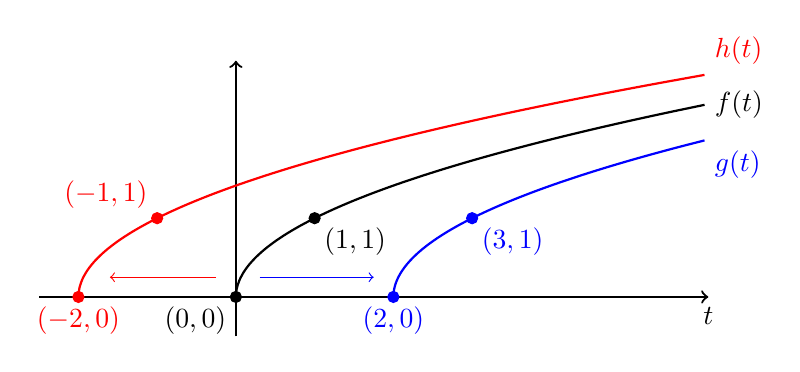
\begin{tikzpicture}
[
	closedpt/.style={circle,draw,fill,inner sep=0pt,minimum size=4pt},
	openpt/.style={circle,draw,inner sep=0pt,minimum size=4pt},
]

	% axes
	\draw[->,thick] (\xmin,0) -- (\xmax,0) node[below] {$t$};
	\draw[->,thick] (0,\ymin) -- (0,\ymax);

	% graph
	\draw[thick, domain=0:2.44, smooth] plot ({\x * \x},\x) node[right] {$f(t)$};
	\draw[thick, blue, domain=0:1.988, smooth, xshift=2cm] plot ({\x * \x},\x) node[below right] {$g(t)$};
	\draw[thick, red, domain=0:2.82, smooth, xshift=-2cm] plot ({\x * \x},\x) node[above right] {$h(t)$};

	\node[closedpt] at (0,0) (orig0) {};
	\node[closedpt] at (1,1) (orig1) {};
	\node[closedpt,blue] at (2,0) (right0) {};
	\node[closedpt,blue] at (3,1) (right1) {};
	\node[closedpt,red] at (-2,0) (left0) {};
	\node[closedpt,red] at (-1,1) (left1) {};

	\node[below left] at (orig0) {$(0,0)$};
	\node[below,blue] at (right0) {$(2,0)$};
	\node[below,red] at (left0) {$(-2,0)$};

	\node[below right] at (orig1) {$(1,1)$};
	\node[below right,blue] at (right1) {$(3,1)$};
	\node[above left,red] at (left1) {$(-1,1)$};

	\draw[->,blue] (0.3,0.25) -- (1.75,0.25);
	\draw[->,red] (-0.25,0.25) -- (-1.6,0.25);

\end{tikzpicture}
